
\subsection{Moyenne :}\label{subsec:moy}
Il a été demandé au réseau de régresser une fonction moyenne à deux dimensions :
Les poids qui sont censés être obtenus sont les suivants :
\begin{equation}
    \label{eq:moy}
    m(X) =\frac{x_1 + x_2}{2} = 0.5 \times x_1 + 0.5 \times x_2
\end{equation}

Le graphique à trois dimensions des valeurs attendues (gauche) et obtenues (droite) est le suivant :
\begin{figure}[H]
    \center
    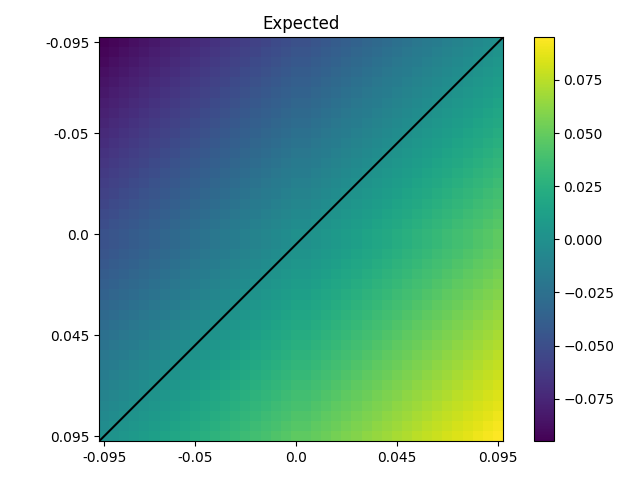
\includegraphics[height=\petit]{pict/moy/expected}
    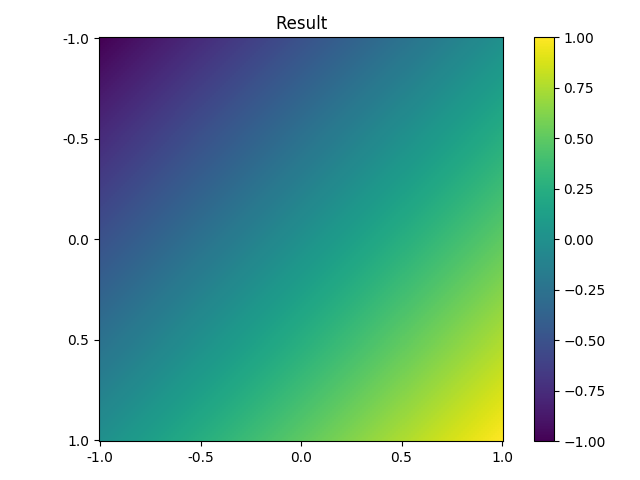
\includegraphics[height=\petit]{pict/moy/result}
	\caption{Apprentissage de la moyenne}
    \vspace{-10pt}
    \begin{center}
        \tiny
        \textit{
        Les axes $x$ et $y$ correspondent respectivement à $x_1$ et $x_2$.
        La valeur en tout point de la fonction est représentée par un gradient de couleur
        dont l'échelle est sur la droite du graphique.
        }
    \end{center}
	\label{fig:moy}
\end{figure}
\vspace{-12pt}

Aucune différence n'est visible, en effet les poids associés aux deux noeuds sont les suivants :
\begin{equation*}
    w_1 = 0.50000010
    \;\;\;\;\;\;\;\;\;
    w_2 = 0.50000024
\end{equation*}
Aux approximations processeur, les poids sont les mêmes que dans (\ref{eq:moy}).


\subsubsection{Étude de l'apprentissage :}\label{subsec:app}
Théoriquement, l'écart type de l'erreur d'apprentissage devrais
diminuer quand la taille de la base de données augmente.
Pour tester cette hypothèse, des graphiques ont été générés avec
différentes tailles de base de données :

\begin{figure}[H]
    \center
    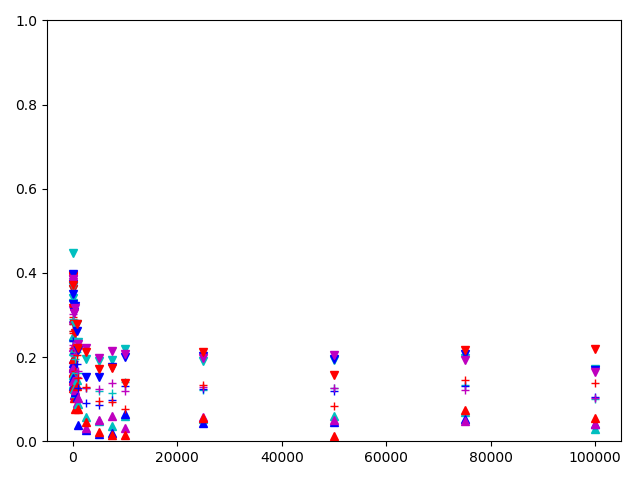
\includegraphics[height=\moyen]{pict/appfd.png}
	\caption{Écart type de l'apprentissage en fonction de la taille de la base de données}
	\label{fig:etfdata2graph}
\end{figure}
\vspace{-5pt}
Ici, l'erreur d'apprentissage s'amoindrit avec l'augmentation de la taille de la base de données.
Cette évolution s'arête vers les $1000$ données, dépassé ce cap, l'écart type stagne.


Un graphique a taille de base de données fixée de l'écart type de l'apprentissage
en fonction du nombre d'apprensitssages réalisés par le réseau.
Cette technique permet de ne pas stagner dans un minimum local.

\begin{figure}[H]
    \center
    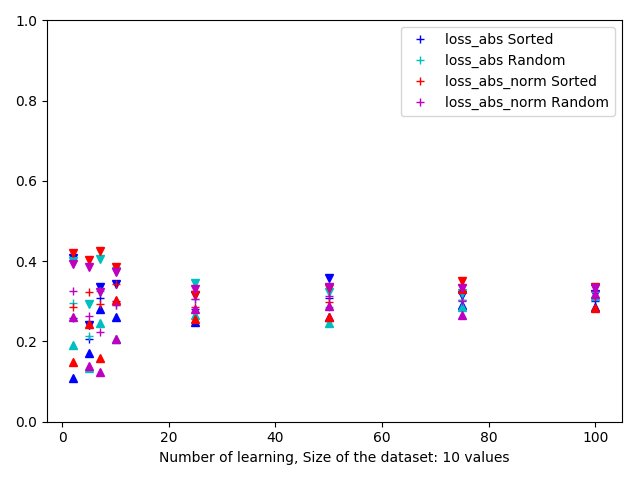
\includegraphics[height=\moyen]{pict/appfn.png}
	\caption{écart type de l'apprentissage moyen en fonction du nombre d'apprensitssages}
	\label{fig:etfngraph1}
\end{figure}
\vspace{-5pt}
Ici, contrairement à la \textsc{Figure}\ \ref{fig:etfdata2graph}, la moyenne ne varie pas significativement mais l'écart type diminue drastiquement.
Ce paramètre combiné au précédent permettra d'augmenter la précision du réseau dans la partie\ \ref{subsec:real}.


\subsection{Étude de la resistance aux perturbations}\label{subsec:random}
Le réseau essaye de régresser une fonction toute simple:
\begin{equation}
    \frac{1}{3} \times x + \frac{2}{3} \times y
\end{equation}
Ici, les poids $1/3$ et $2/3$ ont été choisit pour casser la simétrie.
Une perturbation random équiprobable entre $-err$ et $err$ est ajouté aux données.
Voici un graphique de l'erreur de l'apprentissage en fonction de cette erreur
(allant de $0$ à $\pm$ le maximum de la fonction) :
\begin{figure}[H]
    \center
    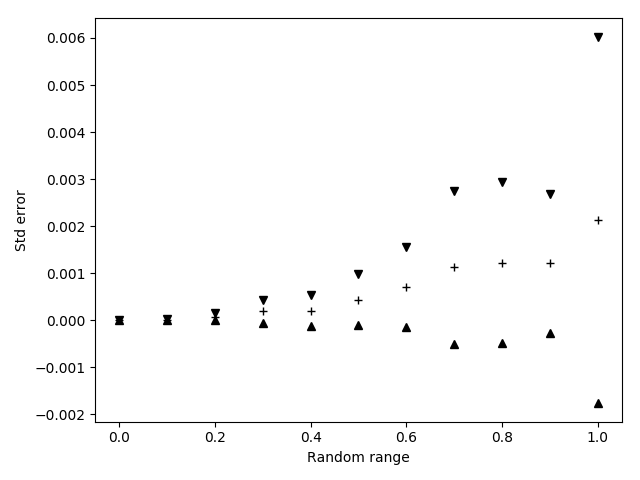
\includegraphics[height=\moyen]{pict/random.png}
	\caption{Variation d'apprensitssage en fonction de la perturbation}
	\label{fig:obj2tiers1}
\end{figure}

Même si l'erreur moyenne augmente exponentiellement avec la perturbation,
elle reste extremement faible $R^2 > 0.99$.

Cet exemple illustre très bien l'extrême robustesse des réseaux de neurones aux perturbations.
Ce réseau n'auras donc pas trop de mal à apprendre sur des données réelles (souvent très ébruitées).


\subsection{Base de données réelle}\label{subsec:real}
Les données ont été passées dans un réseau de neurones sans traitement specifique.
Voici le résultat de l'apprentissage:

\begin{figure}[H]
    \center
    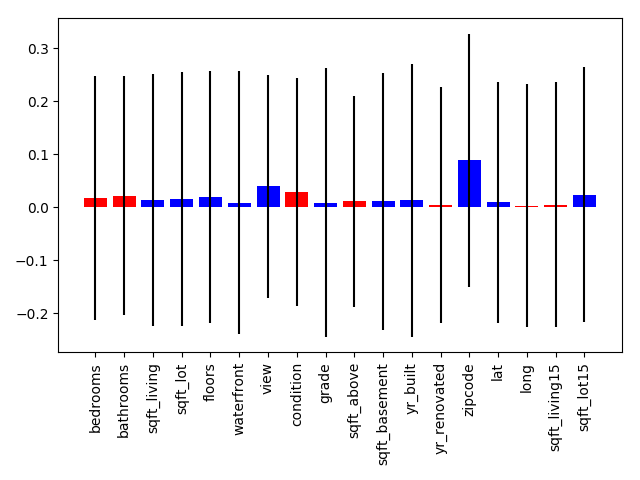
\includegraphics[height=\petit]{pict/real/res1.png}
    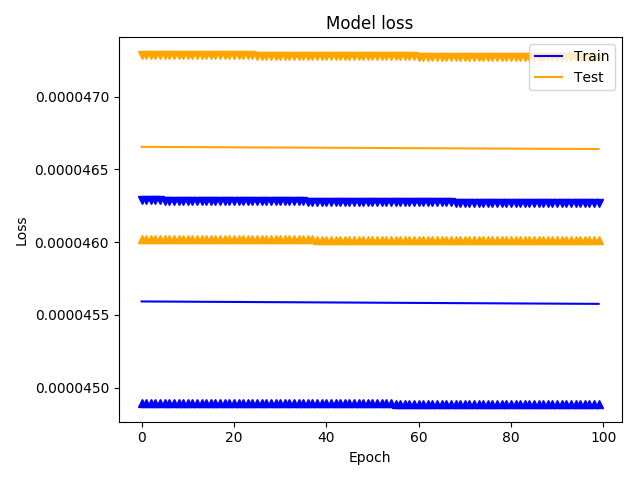
\includegraphics[height=\petit]{pict/real/learn1.png}
	\caption{Apprentissage sur les données réelles}
	\label{fig:def_100_100}
\end{figure}
L'apprentissage est ici totalement cahotique.
Ce résultat était attendu étant donné que les fonctions d'utilité n'ont pas été
calculées et que le prix d'une maison n'est pas un calcul simple.
Ici, il est impossible de calculer le prix avec un simple $Surface \times Prix/m^3$.\\


Les fonctions d'utilités ont donc été calcullées.
Voici le résultat :
\begin{figure}[H]
    \center
    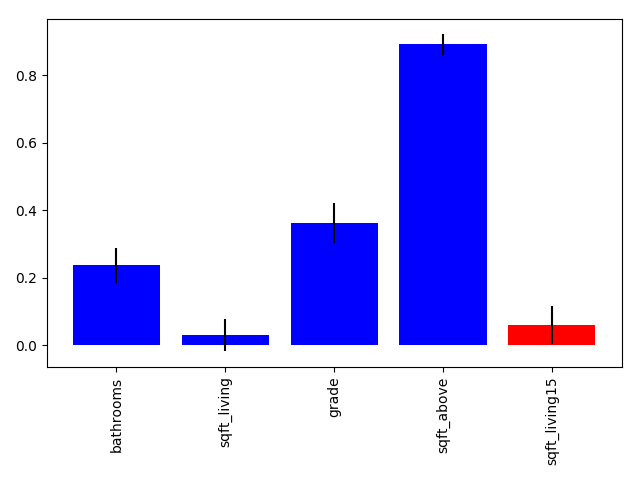
\includegraphics[height=\petit]{pict/real/resut.png}
    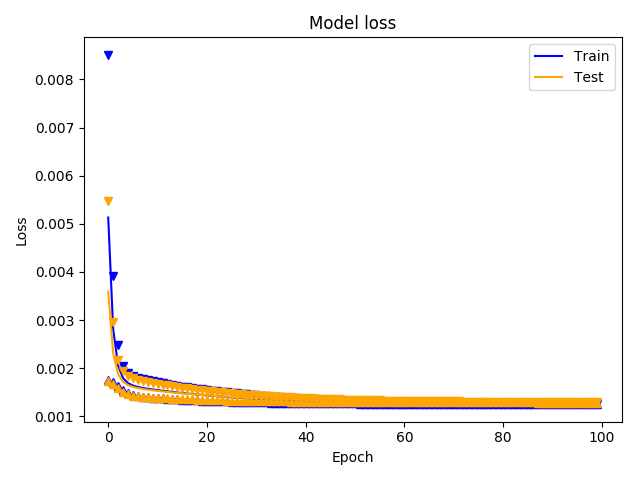
\includegraphics[height=\petit]{pict/real/learnut.png}
	\caption{Apprentissage sur les données réelles}
	\label{fig:ut1_100_100}
\end{figure}
Il peut être remarqué peut que l'apprentissage est bien plus précis.
En effet, l'espace des poids étant bien plus restreint,
le réseau explore cet espace bien plus rapidement.


Les résultats sont donc passés dans un réseau de Choquet afin d'en calculer tout ces coefficients :
\begin{figure}[H]
    \center
    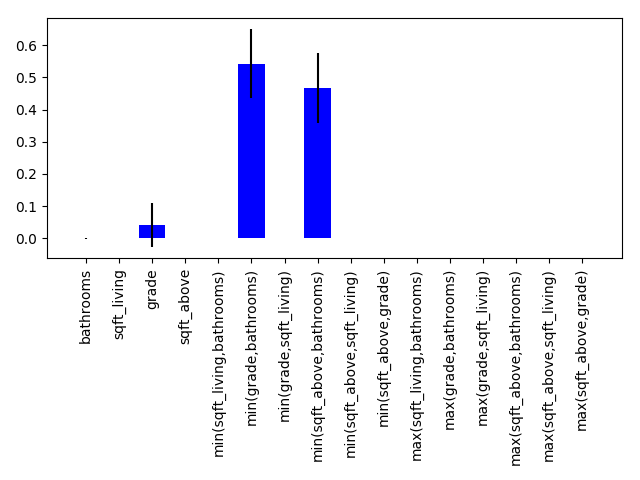
\includegraphics[height=\moyen]{pict/real/netch.png}
    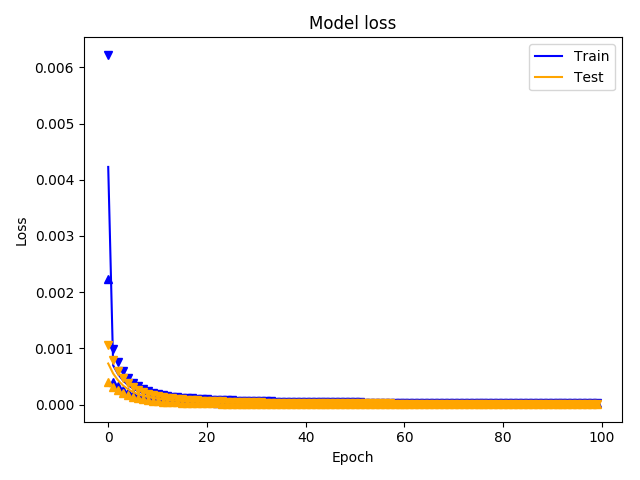
\includegraphics[height=\petit]{pict/real/learnch.png}
	\caption{Apprentissage avec le réseau de Choquet}
	\label{fig:real-Choquet}
\end{figure}

En observant la \textsc{Figure}\ \ref{fig:real-Choquet}, il est visible que seul deux paramètres
ont des valeurs significativement différentes de $0$.
Ces paramètres sont les suivants :
\begin{itemize}
    \item[min(note, nombre de salles de bains) :] La note est un indicateur donné par l'état sur le niveau de la maison.\\
        Et les maisons ayant beaucoup de salles de bains sont plus cheres dans cette base de données.
    \item[min(superficie, nombre de salles de bains) :] La taille de la maison est donc prise en compte,
        mais ce n'est pas le facteur déterminant pour donner un prix à une maison.
\end{itemize}


